\documentclass[runningheads]{venue/lncs/llncs}

\usepackage{amsmath,amssymb}
\usepackage{booktabs}
\usepackage{graphicx}
\usepackage{longtable}
\usepackage{pdflscape}
\usepackage{array}
\usepackage{microtype}
\usepackage[table]{xcolor}
\usepackage{url}
\emergencystretch=2em
\newcolumntype{P}[1]{>{\raggedright\arraybackslash\hfuzz=10pt\relax}p{#1}}
\newcommand{\WS}{W+S}
\newcommand{\runvals}[3]{\shortstack{#1\\#2\\#3}}

\title{Supplementary Material: Deployment-Conditioned Behavioural Diagnostics for Knowledge Transfer}
\titlerunning{Supplementary Material}
\author{Anonymous}
\authorrunning{Anon}
\institute{Anonymous Institution}

\begin{document}
\maketitle

\section{Scope}

This supplement provides reproducibility details, run-level prediction results, common-sample construction, explanation-quality checks, and additional agricultural cases. The main study concerns CY-Bench US-maize-to-Australian-wheat transfer under complete-input GROUP and SPATIAL contracts. Roseworthy E5 examines point-level modality availability; random forest (RF) and privileged-information studies compare training routes, and Waite compares temporal-forward and plot-group protocols. Each study uses its native sample unit and analysis setting.

The evaluated source routes comprise supervised transfer and four knowledge-distillation (KD) variants. Predictive performance is reported as mean absolute error (MAE), root mean squared error (RMSE), and coefficient of determination ($R^2$), subject to the metrics available for each study.

\section{Experiment Overview}

Table~\ref{tab:experiment-map} summarises the study components. Sample units, targets, feature interfaces, and deployment settings remain distinct across rows.

\begin{landscape}
\small
\setlength{\tabcolsep}{3pt}
\renewcommand{\arraystretch}{1.12}
\begin{longtable}{p{3.2cm}p{6.4cm}p{7.0cm}}
\caption{Study overview. Each row states the setting, methods, and connection to the research questions.}\label{tab:experiment-map}\\
\toprule
Study component & Setting and methods & Connection to the paper\\
\midrule
\endfirsthead
\toprule
Study component & Setting and methods & Connection to the paper\\
\midrule
\endhead
Earlier split comparisons & Region-year and trial-specific crop data. Random/interpolation, group, spatial, temporal, spatial--temporal, unseen-location, environment, and hybrid holdouts; empirical model comparisons are separated from oracle diagnostics. & Motivates explicit deployment contracts because model selection can change within a study. Datasets, model spaces, and metrics differ, so these rows are not pooled.\\
US-maize $\rightarrow$ Australian-wheat transfer & CY-Bench regional crop-year yield with ten weather features. Complete-input GROUP and SPATIAL contracts; scratch, supervised, prediction-KD, representation-KD, combined-KD, and missing-aware routes across three runs. & Primary study. Prediction KD improves SPATIAL MAE and produces negative transfer under GROUP. The SPATIAL test has 31 observations and one fixed scratch reference.\\
Common-sample behaviour & Australian-wheat sample clusters with four disjoint weather groups. Permutation SHapley Additive exPlanations (SHAP), signed redistribution, matched error change, and attribution--error comparisons align route, contract, run, feature order, preprocessing, and background. & Relates changes in information use to matched prediction errors. Attribution depends on its background, and the pooled association varies by run.\\
Stress and explanation quality & The same target models under training-median group replacement, nearest-neighbour and 9D Ledoit--Wolf distance, Integrated Gradients (IG) completeness, and local Taylor reconstruction. & Compares stress and attribution rankings and establishes the valid range of the local diagnostics.\\
Local missing-modality RF & Australian-wheat yield with weather and soil inputs under complete, random-missing, and no-weather conditions; joint-feature, branch-average, and single-modality RF controls. & Compares standard feature concatenation with branch-based local baselines under changing input availability.\\
Privileged-information teacher--student & Weather-only Australian-wheat student with complete-input teacher under GROUP/no-soil; observed-target, pseudo-target, and fixed-blend controls. & Compares supervision combinations across runs; the blend has the lowest mean and wins both pairwise controls in S1.\\
Roseworthy E5 & Within-paddock point-level yield; complete-input and soil-unavailable spatial settings with scratch, supervised source initialisation, and four KD-based source-initialised routes. & Relates transfer value to deployment-time modality availability at within-paddock scale.\\
Waite historical case & Single-station historical trial setting with temporal-forward and plot-group protocols. & Relates observed performance to protocol choice when soil descriptors are constant or near-constant.\\
\bottomrule
\end{longtable}
\end{landscape}

\section{Notation and Route Coefficients}

Route, contract, run, target sample, feature, and feature group are indexed by $r$, $c$, $s$, $i$, $j$, and $G$. The symbols $f_{r,c,s}$, $\mathbf{x}_i$, $y_i$, $\boldsymbol{\phi}_i$, and $\mathcal{B}_{c,s}$ denote the adapted target model, input, target, attribution vector, and test-disjoint development background. The source objective is $\mathcal{L}_r=\mathcal{L}_{\rm sup}+\lambda_{\rm pred}^{(r)}\mathcal{L}_{\rm pred}+\lambda_{\rm repr}^{(r)}\mathcal{L}_{\rm repr}+\lambda_{\rm cons}^{(r)}\mathcal{L}_{\rm cons}$. The fitted target model is always adapted with observed target labels; no target-side KD is used.

\begin{table}[h]
\centering
\caption{Evaluation notation used throughout the manuscript and supplement.}
\small
\setlength{\tabcolsep}{3pt}
\begin{tabular}{p{.28\textwidth}p{.62\textwidth}}
\toprule
Symbol & Meaning and unit\\
\midrule
$\mathcal I_{c,s}, n_{c,s}$ & Fixed contract--run test set and its size\\
$e_i^{r,c,s},\Delta e_i^{r,c,s}$ & Absolute error and route-minus-supervised matched error change (t/ha)\\
$\boldsymbol\phi_i^{r,c,s}$ & Attribution vector under test-disjoint development background $\mathcal B_{c,s}$\\
$p_{i,G}^{r,c,s},\Delta p_{i,G}^{r,c,s}$ & Absolute attribution share and route-minus-supervised share change\\
$d_{\phi,i}^{r,c,s}$ & $L_1$ attribution redistribution magnitude\\
$\Delta\phi_{ij}^{r,c,s}$ & Signed route-minus-supervised feature attribution change\\
$q_G^{r,c,s}$ & Prediction change per standardised perturbation distance\\
\bottomrule
\end{tabular}
\end{table}

\paragraph{Run labels.} The three prespecified runs use S1$=101$, S2$=202$, and S3$=303$. These labels identify training runs; repeated target rows are still clustered by sample identifier for inference.

\section{Source Pretraining, Teacher Construction, and Checkpoint Selection}

The source split is temporal and identical across runs. US-maize observations from 2001--2021 form the training set (35,282 region--years), 2022 forms validation (1,512), and 2023 is a source test set (1,430). Median imputation and standardisation are fitted on the 2001--2021 rows only. Source validation selects checkpoints; the 2023 source test and all Australian target data are excluded from selection.

Each non-supervised route and run trains its own teacher from random initialisation. The teacher contains the same 128-dimensional weather encoder used by the student, plus a three-variable soil branch, a fusion layer, and a regression head. It is fitted to observed source yield with mean squared error (MSE) and selected by source-validation MSE. The teacher is then placed in evaluation mode and all of its parameters are frozen. It never receives Australian target data.

The route student is a randomly initialised weather-only model. Prediction KD matches teacher predictions, while representation KD matches the teacher's 128-dimensional fused representation to the student's 128-dimensional weather representation. Combined KD uses both terms. The experimental missing-aware route masks 20\% of standardised weather entries independently within each training batch, represents them as unavailable tokens, and penalises disagreement with the unmasked prediction. The student checkpoint is the epoch with the lowest source-validation MSE, with improvements smaller than $10^{-8}$ treated as ties. Each route--run checkpoint is used only to initialise its corresponding target model.

Target adaptation fits a new target-fold imputer and scaler on target training rows, then optimises supervised MSE. The selected target checkpoint has the lowest validation MSE. Target test rows are evaluated only after selection. There is no target-side teacher prediction or distillation loss. Route-to-route comparisons are run-matched. The SPATIAL scratch comparison instead uses one fixed local reference shared by the transferred runs, so it does not provide three independent scratch replicates.

Permutation SHAP backgrounds contain the first 32 non-test rows in dataset order after median imputation with the matching training-fold preprocessor. The background is fixed across routes within a contract and run. It is test-disjoint but not always training-only: GROUP backgrounds contain 23/32, 32/32, and 9/32 training rows for S1--S3, with the remainder from validation; each SPATIAL background contains 23 training and 9 validation rows. Validation covariates enter this post-hoc background but do not affect model fitting or checkpoint selection; the reference distribution is therefore the target development pool.

\begin{table}[h]
\centering
\caption{Source-route coefficients and training roles.}
\small
\begin{tabular}{lrrrll}
\toprule
Route & $\lambda_{\rm pred}$ & $\lambda_{\rm repr}$ & $\lambda_{\rm cons}$ & Teacher & Target adaptation\\
\midrule
Supervised & 0 & 0 & 0 & no & supervised\\
Prediction KD & 0.5 & 0 & 0 & frozen & supervised\\
Representation KD & 0 & 0.25 & 0 & frozen & supervised\\
Combined KD & 0.5 & 0.25 & 0 & frozen & supervised\\
Missing-aware & 0.25 & 0 & 0.25 & frozen & supervised\\
\bottomrule
\end{tabular}
\end{table}

\section{Early Split-Selection Motivation}\label{sec:early-split}

The earlier comparisons motivate the deployment questions. They combine heterogeneous datasets, model sets, and deployment axes and remain separate from the three-run transfer study.

{\scriptsize
\begin{longtable}{p{2.25cm}p{1.8cm}p{1.65cm}p{1.65cm}p{2.4cm}}
\caption{Empirical model comparisons underlying the partition motivation. Native metrics and units remain attached to each row.}\label{tab:early-empirical}\\
\toprule
Track & Axis & Random winner & Deployment winner & Comparison type\\
\midrule
\endfirsthead
\toprule
Track & Axis & Random winner & Deployment winner & Comparison type\\
\midrule
\endhead
Australian regional & State holdout & HGB & RF & empirical comparison\\
Australian regional & Temporal & HGB & RF & empirical comparison\\
CY-Bench maize US & Spatio-temporal & RF & HGB & empirical comparison\\
CY-Bench maize US & Temporal & RF & HGB & empirical comparison\\
CY-Bench maize US & Unseen location & RF & RF & empirical comparison\\
CY-Bench wheat US & Spatio-temporal & HGB & HGB & empirical comparison\\
CY-Bench wheat US & Temporal & HGB & HGB & empirical comparison\\
CY-Bench wheat US & Unseen location & HGB & HGB & empirical comparison\\
\bottomrule
\end{longtable}
}

{\scriptsize
\begin{longtable}{p{2.25cm}p{1.8cm}p{1.65cm}p{1.65cm}p{2.4cm}}
\caption{Diagnostic and oracle comparisons. These rows are non-deployable diagnostics and are not prevalence estimates.}\label{tab:early-diagnostic}\\
\toprule
Track & Axis & Random selector & Deployment selector & Comparison type\\
\midrule
\endfirsthead
\toprule
Track & Axis & Random selector & Deployment selector & Comparison type\\
\midrule
\endhead
CY-Bench fixed & Spatio-temporal & Gate & Oracle & diagnostic/oracle\\
CY-Bench fixed experts & Temporal & Gate & Best single & diagnostic/oracle\\
CY-Bench fixed experts & Unseen location & Gate & Best single & diagnostic/oracle\\
G2F native & Temporal & Oracle & Oracle & diagnostic/oracle\\
G2F native & Unseen environment & Oracle & HGB & diagnostic/oracle\\
G2F native & Unseen hybrid & Oracle & HGB & diagnostic/oracle\\
\bottomrule
\end{longtable}
}

HGB denotes histogram gradient boosting. Gate is a model-selection diagnostic, Oracle is a non-deployable selector, and Best single is the strongest eligible single model. The empirical rows use conventional linear and tree baseline families adapted to their respective data interfaces. The diagnostic rows distinguish deployable comparisons from selection thought experiments. Each comparison keeps its native metric and unit.

\subsection{Early candidate models and their relation to CY-Bench}

Table~\ref{tab:early-models} identifies the model families represented in the earlier comparisons. Candidate sets vary by dataset and split. The fixed references and tabular models use a CY-Bench-compatible regional interface, while some additional families appear only in selected comparisons.

{\scriptsize
\begin{longtable}{p{2.8cm}p{3.0cm}p{5.7cm}}
\caption{Model families and diagnostic selectors in the earlier split comparisons. ``Present'' indicates availability within the relevant comparison, whose candidate set may vary by dataset.}\label{tab:early-models}\\
\toprule
Family or selector & Classification & Use in the earlier material\\
\midrule
\endfirsthead
\toprule
Family or selector & Classification & Use in the earlier material\\
\midrule
\endhead
Average-yield and linear-trend references & CY-Bench-inspired fixed baselines & Used on the CY-Bench-compatible tabular interface; not verbatim official implementations.\\
Ridge and other regularised linear candidates & Additional baselines & Ridge has empirical comparison rows. Linear, lasso, and elastic-net estimators occur in the comparison material but are not part of the earlier ranking table.\\
Random forest and HGB & Additional tree/boosting baselines & Empirical comparisons use the specified tabular protocol.\\
XGBoost & Adapted from a CY-Bench-compatible prediction protocol & XGBoost predictions were available for selected CY-Bench comparisons, but the model was not retrained within that comparison set.\\
LightGBM and SVR & Additional baselines & Present in the comparison material but absent from the empirical ranking comparisons.\\
Kernel-ridge RBF & Additional literature comparator & Evaluated only on an auxiliary G2F setting; it is not part of the early CY-Bench ranking comparisons.\\
LSTM & Additional deep baseline & Present in the comparison material. Its documented result is diagnostic, so it is excluded from empirical ranking claims.\\
Mean, weighted, and stacking ensembles & Additional ensembles & Used in selected fixed-expert comparisons.\\
Gate, Oracle, and Best single & Non-deployable diagnostics & Selection thought experiments or reference selectors. They are separated from empirical model comparisons and do not estimate deployable model ranking.\\
\bottomrule
\end{longtable}
}

\section{Data, Features, and Splits}

The source comprises 38,224 US maize region--year observations from 2,307 regions; the Australian wheat target comprises 490 region--year observations from 25 regions. Both cover 2001--2023 and use tonnes per hectare. The feature interface and target definitions follow CY-Bench and related crop-yield modelling work \cite{Kallenberg2026CYBench,Khaki2019DNNYield}.

The ten analysed weather features, in model order, are observed days, expected days, coverage, mean minimum temperature, mean maximum temperature, precipitation sum, accumulated radiation, reference evapotranspiration, vapour-pressure deficit, and climatic water balance. The first three form the observation-support group. Temperature contains the next two; water balance contains precipitation, evapotranspiration, vapour-pressure deficit, and climatic water balance; radiation is a separate group. These four groups are mutually exclusive. Constant coverage is excluded from covariance-based out-of-distribution (OOD) distance.

GROUP applies two run-seeded group-shuffle operations: 20\% of administrative groups form the test split and 20\% of the remaining groups form validation. SPATIAL bins latitude and longitude into a $4\times4$ grid, assigns every fifth occupied block to test, and every fourth remaining block to validation. Its assignment is fixed across runs. Partitions are exhaustive and mutually exclusive. All imputation and standardisation parameters are fitted on the corresponding target-training fold.

\section{Architecture, Optimisation, and Source Routes}

Each weather feature is represented as a token containing feature identity, time, standardised value, and availability. A two-layer Transformer encoder \cite{Vaswani2017Transformer} uses embedding width 64, four attention heads, feed-forward width 192, and dropout 0.1. Availability-weighted pooling gives a 128-dimensional representation; the regression head has hidden width 64 with GELU and dropout 0.1.

Training uses AdamW \cite{Loshchilov2019AdamW} with weight decay $10^{-4}$, batch size 256, at most 80 epochs, and early-stopping patience 12. Source training and target scratch use learning rate $10^{-3}$; transferred target fine-tuning uses $2\times10^{-4}$. Teacher, source-student, and target checkpoints minimise validation MSE. Checkpoint selection records squared validation RMSE after aggregating predictions over the full validation set, which is numerically identical to MSE. Source-route losses are:
\[
\begin{array}{ll}
\text{supervised} & L_{\rm sup},\\
\text{prediction KD} & L_{\rm sup}+0.5L_{\rm pred},\\
\text{representation KD} & L_{\rm sup}+0.25L_{\rm repr},\\
\text{combined KD} & L_{\rm sup}+0.5L_{\rm pred}+0.25L_{\rm repr},\\
\text{missing-aware} & L_{\rm sup}+0.25L_{\rm pred}+0.25L_{\rm cons}.
\end{array}
\]
The teacher is frozen for all non-supervised source routes. Representation matching compares the teacher's 128-dimensional fused representation with the student's 128-dimensional weather representation. Target adaptation always uses observed target labels and supervised MSE; there is no target-side KD.

\section{Empirical Results}

\begin{longtable}{lllrrrr}
\caption{Primary target-test results. Metrics are computed on the same test rows within each contract and run. The SPATIAL scratch value is one fixed local reference, not a three-run variance estimate.}
\label{tab:full-performance}\\
\toprule
Contract & Route & Seed & $n$ & MAE & RMSE & $R^2$\\
\midrule
\endfirsthead
\toprule
Contract & Route & Seed & $n$ & MAE & RMSE & $R^2$\\
\midrule
\endhead
GROUP & Scratch & S1 & 94 & 0.673 & 0.885 & 0.337\\
& Scratch & S2 & 115 & 0.700 & 0.869 & -0.596\\
& Scratch & S3 & 93 & 0.814 & 1.002 & 0.395\\
& Supervised & S1 & 94 & 1.049 & 1.236 & -0.294\\
& Supervised & S2 & 115 & 0.666 & 0.821 & -0.424\\
& Supervised & S3 & 93 & 1.009 & 1.224 & 0.097\\
& Prediction KD & S1 & 94 & 1.592 & 2.304 & -3.500\\
& Prediction KD & S2 & 115 & 0.859 & 1.087 & -1.494\\
& Prediction KD & S3 & 93 & 1.019 & 1.194 & 0.140\\
& Combined KD & S1 & 94 & 0.816 & 1.005 & 0.144\\
& Combined KD & S2 & 115 & 0.677 & 0.871 & -0.601\\
& Combined KD & S3 & 93 & 1.018 & 1.241 & 0.071\\
& Representation KD & S1 & 94 & 0.904 & 1.090 & -0.007\\
& Representation KD & S2 & 115 & 0.806 & 0.999 & -1.108\\
& Representation KD & S3 & 93 & 1.135 & 1.377 & -0.144\\
& Missing-aware & S1 & 94 & 0.830 & 1.012 & 0.131\\
& Missing-aware & S2 & 115 & 0.731 & 0.934 & -0.843\\
& Missing-aware & S3 & 93 & 0.968 & 1.164 & 0.184\\
\midrule
SPATIAL & Scratch & fixed reference & 31 & 1.204 & 1.594 & -0.970\\
& Supervised & S1 & 31 & 0.989 & 1.101 & 0.060\\
& Supervised & S2 & 31 & 1.165 & 1.415 & -0.552\\
& Supervised & S3 & 31 & 0.918 & 1.126 & 0.017\\
& Prediction KD & S1 & 31 & 0.833 & 1.065 & 0.121\\
& Prediction KD & S2 & 31 & 1.140 & 1.447 & -0.622\\
& Prediction KD & S3 & 31 & 0.889 & 1.053 & 0.141\\
& Combined KD & S1 & 31 & 1.118 & 1.276 & -0.262\\
& Combined KD & S2 & 31 & 0.962 & 1.071 & 0.111\\
& Combined KD & S3 & 31 & 0.875 & 1.116 & 0.034\\
& Representation KD & S1 & 31 & 0.973 & 1.070 & 0.113\\
& Representation KD & S2 & 31 & 1.142 & 1.442 & -0.611\\
& Representation KD & S3 & 31 & 0.925 & 1.193 & -0.104\\
& Missing-aware & S1 & 31 & 0.894 & 1.084 & 0.089\\
& Missing-aware & S2 & 31 & 1.281 & 1.508 & -0.764\\
& Missing-aware & S3 & 31 & 1.107 & 1.384 & -0.486\\
\bottomrule
\end{longtable}

Prediction KD improves SPATIAL MAE relative to the fixed scratch reference by 0.371, 0.064, and 0.315~t/ha across S1--S3. Relative to run-matched supervised transfer, the differences are $-0.156$, $-0.025$, and $-0.029$. Under GROUP, prediction-KD differences from scratch are $+0.919$, $+0.159$, and $+0.205$, establishing negative transfer against the local target reference \cite{Wang2019NegativeTransfer}. The repeated SPATIAL scratch value is a fixed local reference reused across these comparisons, not an estimate of seed variability.

The following tables present each modality comparison and agricultural setting separately. A dash denotes an unavailable quantity, not zero. Metrics are in t/ha unless stated otherwise.


\begin{table}[htbp]
\centering
\small
\caption{Roseworthy E5 within-paddock results. The transferred routes use source checkpoints trained on CY-Bench US maize; ``Sup. init.'' denotes supervised source-initialised fine-tuning.}\label{tab:roseworthy-results}
\setlength{\tabcolsep}{3pt}
\renewcommand{\arraystretch}{1.08}
\textbf{(a) Complete-input spatial setting}\\[2pt]
\begin{tabular}{@{}P{1.55cm}P{1.55cm}rrrP{1.0cm}rP{1.35cm}@{}}
\toprule
Route & Inputs & MAE & RMSE & $R^2$ & Ref. & $\Delta$MAE & Finding\\
\midrule
Scratch & full/full & 0.465 & 0.637 & 0.131 & -- & 0.000 & local\\
Sup. init. & full/full & 0.465 & 0.637 & 0.133 & scratch & -0.000 & parity\\
Pred. KD & full/full & 0.470 & 0.641 & 0.122 & scratch & +0.004 & no gain\\
Repr. KD & full/full & 0.473 & 0.644 & 0.112 & scratch & +0.008 & no gain\\
Comb. KD & full/full & 0.466 & 0.637 & 0.133 & scratch & +0.000 & parity\\
Missing & full/full & 0.468 & 0.639 & 0.125 & scratch & +0.003 & no gain\\
\bottomrule
\end{tabular}

\medskip
\textbf{(b) No-soil deployment setting}\\[2pt]
\begin{tabular}{@{}P{1.55cm}P{1.55cm}rrrP{1.0cm}rP{1.35cm}@{}}
\toprule
Route & Inputs & MAE & RMSE & $R^2$ & Ref. & $\Delta$MAE & Finding\\
\midrule
Scratch & full/W & 0.499 & 0.667 & 0.049 & -- & 0.000 & local\\
Sup. init. & full/W & 0.465 & 0.637 & 0.133 & scratch & -0.034 & MAE lower\\
Pred. KD & full/W & 0.470 & 0.641 & 0.122 & scratch & -0.029 & MAE lower\\
Repr. KD & full/W & 0.473 & 0.644 & 0.112 & scratch & -0.026 & MAE lower\\
Comb. KD & full/W & 0.466 & 0.637 & 0.133 & scratch & -0.033 & MAE lower\\
Missing & full/W & 0.468 & 0.639 & 0.125 & scratch & -0.030 & MAE lower\\
\bottomrule
\end{tabular}

\parbox{\textwidth}{\small W denotes weather and S denotes soil.}
\end{table}

\begin{table}[htbp]
\centering
\caption{Local missing-modality random forest (RF) and privileged-information results for Australian wheat region--years. Detailed route results appear in Tables~16--17.}\label{tab:modality-results}
\setlength{\tabcolsep}{1.5pt}
\renewcommand{\arraystretch}{1.12}
\textbf{(a) Local missing-modality RF}\\[2pt]
\begin{tabular}{@{}P{1.75cm}P{2.25cm}P{0.85cm}P{0.65cm}P{0.85cm}P{2.75cm}P{2.1cm}@{}}
\toprule
Condition & Route & Runs & Test $n$ & MAE & Other metrics & Finding\\
\midrule
Complete & Joint-feature RF mean & S1--S3 & 31 & 0.944 & -- & strongest tested RF\\
15\% random missing & Joint-feature RF mean & S1--S3 & 31 & 0.920 & RMSE 1.046; $R^2$ 0.152 & strongest tested RF\\
No weather & All RF variants & S1--S3 & 31 & 1.024 & -- & branch tie\\
\bottomrule
\end{tabular}

\vspace{5pt}
\textbf{(b) Privileged-information teacher--student}\\[2pt]
\begin{tabular}{@{}P{2.15cm}P{0.85cm}P{3.25cm}P{0.75cm}P{2.95cm}@{}}
\toprule
Route & Runs & MAE by run & Mean & Finding\\
\midrule
Observed-target only & S1--S3 & 0.935; 0.580; 0.863 & 0.793 & run-sensitive\\
Pseudo-target only & S1--S3 & 0.901; 0.598; 0.880 & 0.793 & run-sensitive\\
Fixed blend & S1--S3 & 0.886; 0.583; 0.871 & 0.780 & lowest mean; beats both controls in one run\\
\bottomrule
\end{tabular}
\parbox{\textwidth}{\small The privileged-information student uses weather at deployment; its teacher uses weather and soil during source training.}
\end{table}

\begin{longtable}{P{1.7cm}P{1.15cm}P{0.85cm}P{1.35cm}P{2.0cm}P{2.1cm}}
\caption{Waite historical protocol comparison. Native MAE values are reported for the three runs.}\label{tab:waite-results}\\
\toprule
Protocol & Unit & Test $n$ & Route & MAE by run & Interpretation\\
\midrule
\endfirsthead
\toprule
Protocol & Unit & Test $n$ & Route & MAE by run & Interpretation\\
\midrule
\endhead
Temporal-forward & station & 272 & RF-light & 0.691; 0.698; 0.685 & protocol\\
Plot-group & station & 256 & RF-light & 0.502; 0.477; 0.499 & protocol\\
\bottomrule
\end{longtable}
\noindent W+S denotes weather plus soil.

\section{Repeated-Sample Construction}

The explanation inputs contain 395 contract--seed sample rows: GROUP contributes 94, 115, and 93 test rows across the three seeds, while SPATIAL repeats the same 31-row test set. These rows correspond to 287 unique sample identifiers: 279 in GROUP, 31 in SPATIAL, with 23 identifiers occurring in both contracts. Five neural routes yield 1,975 model--sample explanations.

Matching first fixes contract, route, run, sample identifier, feature order, preprocessor, and explained target row. Repeated identifiers are then averaged across runs within contract and route, producing sample-cluster observations. Run-specific estimates are reported separately for stability analysis. The cluster-level tests never treat feature rows, checkpoints, or repeated sample--run rows as independent replicates.

Cluster mean intervals use 4,999 bootstrap resamples. Two-sided Spearman permutation tests use 4,999 permutations, and their intervals use 4,999 cluster bootstraps. Deterministic pseudo-random states begin at 20260709 and advance by route--contract cell. The eight attribution--error tests are adjusted together with Holm's procedure.

\section{Observation-Support and Signed Feature Redistribution}

\begin{figure}[tb]
\centering
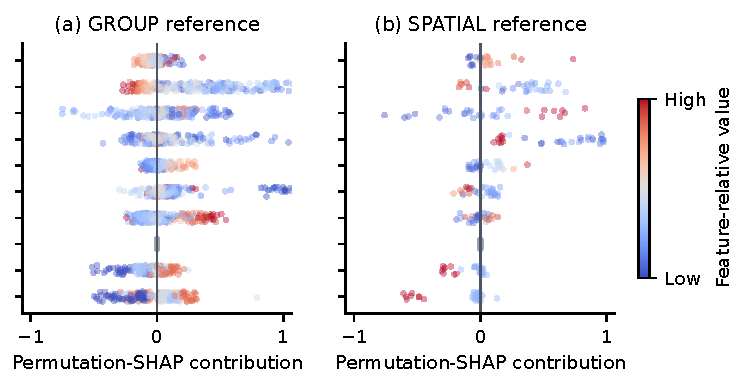
\includegraphics[width=\textwidth]{../figures/final_publication_v4_18/supplement_figure_supervised_landscapes.pdf}
\caption{Descriptive supervised-reference Permutation-SHAP landscapes after repeated identifiers are collapsed across runs to sample clusters. Colour denotes a feature-specific pooled relative value across contracts and is not comparable in absolute units between features; grey marks constant coverage. The GROUP and SPATIAL panels combine fitted-model and test-support differences and are not matched causal contrasts. Obs./Exp. days denote observed/expected days; Cov., Tmin, Tmax, Precip., Rad., ET0, VPD, and WB denote coverage, minimum/maximum temperature, precipitation, radiation, reference evapotranspiration, vapour-pressure deficit, and climatic water balance.}
\label{fig:supervised-landscapes}
\end{figure}

\begin{table}[h]
\centering
\caption{Sample-cluster change in observation-support attribution share relative to supervised transfer. Intervals are 95\% bootstrap intervals.}
\small
\setlength{\tabcolsep}{4pt}
\begin{tabular}{llr@{\hspace{5pt}}r@{\hspace{8pt}}r@{\hspace{8pt}}r}
\toprule
Contract & Route & $n$ & Mean & \multicolumn{1}{c}{Interval} & \multicolumn{1}{c}{Positive}\\
\midrule
GROUP & Prediction KD & 279 & 0.069 & [0.057, 0.082] & 0.720\\
& Combined KD & 279 & 0.078 & [0.065, 0.090] & 0.835\\
& Representation KD & 279 & 0.102 & [0.082, 0.123] & 0.753\\
& Missing-aware & 279 & 0.090 & [0.074, 0.105] & 0.785\\
\midrule
SPATIAL & Prediction KD & 31 & 0.001 & [-0.011, 0.013] & 0.613\\
& Combined KD & 31 & 0.048 & [0.019, 0.075] & 0.677\\
& Representation KD & 31 & -0.004 & [-0.020, 0.011] & 0.516\\
& Missing-aware & 31 & -0.021 & [-0.033, -0.009] & 0.258\\
\bottomrule
\end{tabular}
\end{table}

Figure~\ref{fig:signed-feature} shows signed $\Delta\phi_{ij}^{r,c,s}$ after sample clustering. Directional statements are never inferred from $|\Delta\phi|$; absolute differences are used only for redistribution magnitude. Complete feature-by-route means, medians, intervals, absolute magnitudes, and cluster counts are provided in the accompanying source table.

\begin{figure}[tb]
\centering
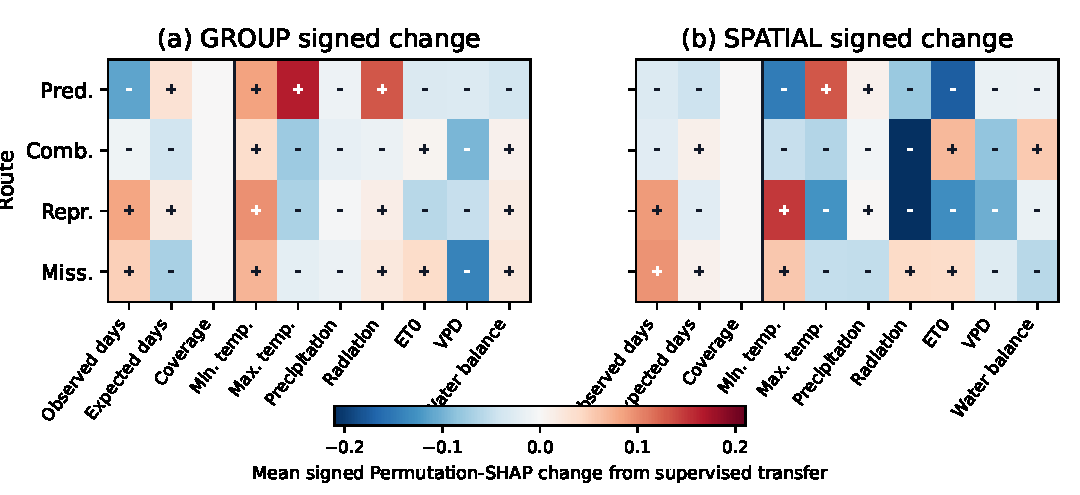
\includegraphics[width=.96\textwidth]{../figures/final_submission_v4_18_5/supplement_figure_s2.pdf}
\caption{Signed feature-level Permutation-SHAP redistribution relative to supervised transfer. GROUP and SPATIAL use the same feature order and colour scale; values are sample-cluster means. Cell symbols show direction: $+$ is positive and $-$ is negative route-minus-supervised mean change. The vertical divider separates observation-support from physical-content features.}
\label{fig:signed-feature}
\end{figure}

\section{Attribution Concentration}

\begin{table}[h]
\centering
\caption{Change in normalised attribution entropy and effective feature count relative to supervised transfer.}
\small
\setlength{\tabcolsep}{4pt}
\begin{tabular}{llrr}
\toprule
Contract & Route & \shortstack{Mean $\Delta$\\entropy} & \shortstack{Mean $\Delta$\\effective features}\\
\midrule
GROUP & Prediction KD & 0.044 & 0.520\\
& Combined KD & 0.055 & 0.722\\
& Representation KD & 0.023 & 0.319\\
& Missing-aware & 0.061 & 0.811\\
\midrule
SPATIAL & Prediction KD & 0.030 & 0.333\\
& Combined KD & 0.056 & 0.705\\
& Representation KD & 0.036 & 0.469\\
& Missing-aware & 0.015 & 0.175\\
\bottomrule
\end{tabular}
\end{table}

All cells broaden rather than concentrate the absolute attribution distribution on average. These smaller effects are descriptive and are not used to interpret the performance reversal.

\section{Attribution--Error Robustness}

\begin{table}[h]
\centering
\caption{Sample-cluster Spearman tests and bivariate trimming sensitivity. Holm correction is applied once to the eight route--contract attribution--error tests.}
\small
\begin{tabular}{llrrrr}
\toprule
Contract & Route & $\rho$ & 95\% bootstrap interval & Holm $p$ & Trimmed $\rho$\\
\midrule
GROUP & Prediction KD & 0.220 & [0.087, 0.338] & 0.0016 & 0.232\\
& Combined KD & -0.112 & [-0.238, 0.016] & 0.407 & -0.132\\
& Representation KD & -0.027 & [-0.155, 0.099] & 1.000 & -0.075\\
& Missing-aware & -0.158 & [-0.280, -0.034] & 0.060 & -0.194\\
\midrule
SPATIAL & Prediction KD & 0.148 & [-0.181, 0.456] & 1.000 & 0.160\\
& Combined KD & -0.012 & [-0.345, 0.352] & 1.000 & -0.042\\
& Representation KD & 0.114 & [-0.344, 0.527] & 1.000 & 0.033\\
& Missing-aware & -0.113 & [-0.438, 0.243] & 1.000 & -0.087\\
\bottomrule
\end{tabular}
\end{table}

Trimming removes observations outside the bivariate 2.5th--97.5th percentiles and is not used for primary inference. GROUP prediction KD remains positive after trimming. Its run-level estimates are 0.415, 0.442, and $-0.274$; leave-one-run-out estimates are 0.111, 0.166, and 0.310. The pooled association is therefore robust to removing any one run, but one run supplies a genuine direction reversal.

Other routes also show seed heterogeneity. GROUP combined-KD single-seed correlations are $-0.370$, 0.197, and 0.016; GROUP missing-aware values are $-0.191$, 0.171, and $-0.097$. SPATIAL prediction-KD values are 0.067, 0.181, and 0.022. These patterns motivate the restricted wording in the main text.

\section{SHAP--IG Agreement and Explanation Quality}

\begin{table}[h]
\centering
\caption{Completeness-qualified sample-cluster SHAP--IG agreement.}
\small
\begin{tabular}{llrrr}
\toprule
Contract & Route & Mean rank $\rho$ & Sign agreement & Top-3 overlap\\
\midrule
GROUP & Supervised & 0.531 & 0.654 & 0.590\\
& Prediction KD & 0.496 & 0.648 & 0.486\\
& Combined KD & 0.429 & 0.618 & 0.472\\
& Representation KD & 0.517 & 0.622 & 0.497\\
& Missing-aware & 0.461 & 0.647 & 0.468\\
\midrule
SPATIAL & Supervised & 0.532 & 0.662 & 0.559\\
& Prediction KD & 0.477 & 0.666 & 0.548\\
& Combined KD & 0.443 & 0.666 & 0.461\\
& Representation KD & 0.614 & 0.646 & 0.559\\
& Missing-aware & 0.553 & 0.612 & 0.557\\
\bottomrule
\end{tabular}
\end{table}

SHAP uses 64 sampled feature-order permutations and the 32-row test-disjoint development background described above. IG uses 64 integration steps from zero in standardised space, corresponding to the training-scaler mean. The 5\% completeness criterion is met by 1,954 of 1,975 explanations (98.9\%). Agreement is moderate and method-dependent; the completeness and local-fidelity checks define how the comparison is interpreted \cite{Hooker2019ROAR,Lundberg2017SHAP,Sundararajan2017IntegratedGradients}.

Pathwise Taylor uses a training-derived reference and a 5\% criterion on the local reconstruction residual. Only 28 of 180 evaluated cases pass (15.6\%). Taylor and Hessian interactions are therefore local diagnostics and are excluded from feature and mechanism claims.

\begin{figure}[tb]
\centering
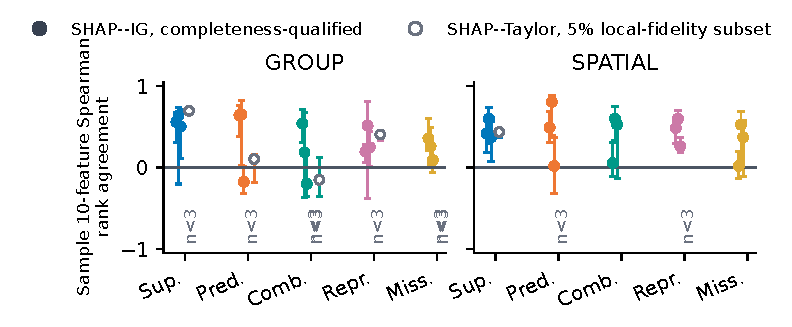
\includegraphics[width=.96\textwidth]{../figures/final_publication_v4_18/supplement_figure_s4.pdf}
\caption{Route--contract--seed explanation-method agreement. Filled markers show completeness-qualified SHAP--IG median within-sample ten-feature Spearman agreement and interquartile range (IQR). Open markers show the 5\% local-fidelity-qualified SHAP--Taylor subset; cells with fewer than three qualified samples are labelled rather than estimated.}
\label{fig:agreement}
\end{figure}

\section{Perturbation and OOD Validity}\label{sec:quality}

\begin{figure}[tb]
\centering
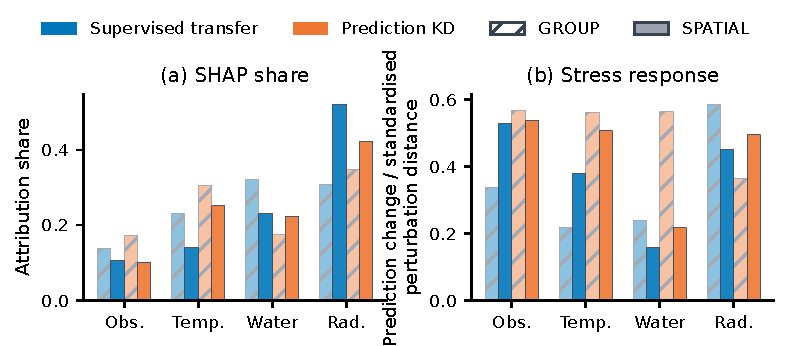
\includegraphics[width=\textwidth]{../figures/final_publication_v4_18/supplement_figure_representative_stress.pdf}
\caption{Representative attribution and finite-stress profiles for supervised transfer and prediction KD. Panels (a--b) use four mutually exclusive groups: observation support, temperature, water balance, and radiation. GROUP uses hatched bars and SPATIAL uses solid bars. Stress is prediction change per standardised perturbation distance and is not feature importance.}
\label{fig:representative-stress}
\end{figure}

\begin{figure}[tb]
\centering
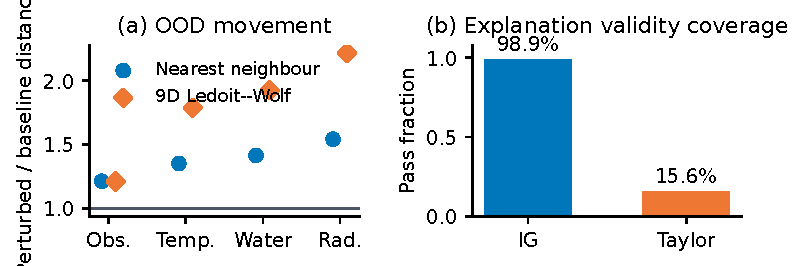
\includegraphics[width=.82\textwidth]{../figures/final_publication_v4_18/figure_06.pdf}
\caption{Validity boundaries for the finite feature-group stress tests. Panel (a) reports perturbed-to-baseline nearest-neighbour and stable nine-dimensional Ledoit--Wolf distance ratios for four discrete groups. Panel (b) reports two different qualification rates: IG completeness and pathwise-Taylor local reconstruction. The gates are not interchangeable; Taylor remains a conditional local diagnostic.}
\label{fig:validity}
\end{figure}

Attribution--stress agreement uses exactly four mutually exclusive groups. Across 30 route--contract--seed cells, mean Spearman agreement is $-0.040$; GROUP and SPATIAL means are 0.067 and $-0.147$. Nine cells (30\%) identify the same top attribution and stress group. Overlapping ``all physical'' or ``all support'' aggregates are not included.

\begin{table}[h]
\centering
\caption{OOD distances averaged across contracts and seeds. Covariance distance uses the nine non-constant standardised dimensions and Ledoit--Wolf shrinkage \cite{LedoitWolf2004}.}
\small
\begin{tabular}{lrrrr}
\toprule
Group & Base NN & Perturbed NN & Base Mah. & Perturbed Mah.\\
\midrule
Observation support & 0.759 & 0.922 & 2.681 & 3.247\\
Temperature & 0.759 & 1.018 & 2.681 & 4.792\\
Water balance & 0.759 & 1.075 & 2.681 & 5.161\\
Radiation & 0.759 & 1.170 & 2.681 & 5.942\\
\bottomrule
\end{tabular}
\end{table}

One GROUP seed has a lower nearest-neighbour distance after observation-support replacement, while the multivariate shrinkage distance and aggregate movement are outward. We interpret the finite tests as controlled stress interventions over this measured distance range \cite{Covert2021Removing,Hase2021OODExplainability}.

\section{Continuous Three-View Route Pairs}

For each route, contract, and seed, the route-pair table reports mean matched error change, fraction of samples improved, mean absolute prediction difference, mean $d_{\phi}$, and mean stress-response difference. For example, SPATIAL prediction KD improves over supervised transfer by 0.156, 0.025, and 0.029 MAE across seeds, while mean attribution distances are 1.996, 2.983, and 1.530 and stress-response differences are 0.135, 0.177, and 0.149. These continuous quantities show that predictive and behavioural proximity can differ.

We omit the earlier 1.5~t/ha high-error-tail threshold because its prediction-row denominator does not match the final common-sample construction. The continuous route-pair quantities preserve one sample-selection rule.

\section{Missing-Modality Comparisons}\label{sec:missing}

\subsection{Joint-feature RF}

The local tree model concatenates weather and soil columns after training-fold median imputation and fits an RF model with 150 trees, minimum leaf size 2, one thread, and a seed-specific random state \cite{Breiman2001RandomForests}. Table~\ref{tab:rf} compares it with weather-only, soil-only, and branch-averaged modality-specific forests under identical SPATIAL contracts.

\begin{table}[h]
\centering
\caption{Local RF mean MAE across three seeds. ``Best branch'' is the lower-error single-modality control.}
\label{tab:rf}
\small
\begin{tabular}{lrrr}
\toprule
Condition & Joint-feature RF & Branch average & Best branch\\
\midrule
Complete & \textbf{0.944} & 1.053 & 1.024\\
15\% random missing & \textbf{0.920} & 1.015 & 1.004\\
No weather & 1.024 & 1.024 & 1.024\\
\bottomrule
\end{tabular}
\end{table}

The joint model is the strongest tested local tree configuration for complete and random-missing inputs. It uses standard feature concatenation and RF fitting. Under no-weather input, all executable variants reduce to the soil-only branch and therefore tie.

\subsection{Privileged-information teacher--student}\label{sec:pi}

A complete-modality RF teacher supplies pseudo-targets to a weather-only MLP with hidden widths 64 and 32. The fixed blend is compared with same-architecture observed-target-only and pseudo-target-only controls, following the learning-with-privileged-information distinction \cite{LopezPaz2016GeneralizedDistillation}.

\begin{table}[h]
\centering
\caption{GROUP/no-soil MAE for all privileged-information seeds.}
\small
\begin{tabular}{lrrr}
\toprule
Seed & Observed target & Pseudo-target & Fixed blend\\
\midrule
S1 & 0.935 & 0.901 & \textbf{0.886}\\
S2 & \textbf{0.580} & 0.598 & 0.583\\
S3 & \textbf{0.863} & 0.880 & 0.871\\
\midrule
Mean & 0.793 & 0.793 & \textbf{0.780}\\
\bottomrule
\end{tabular}
\end{table}

The blend has the lowest mean and beats both controls in S1. The ordering changes in S2 and S3, showing run-level variation in the value of train-time privileged information.

\section{Agricultural Case Studies}\label{sec:secondary-cases}

\subsection{Roseworthy E5 within-paddock evidence}

Roseworthy E5 is a point-level, within-paddock yield setting with 43,311 registered observations from 2007--2008. The transferred routes use checkpoints trained on CY-Bench US maize before target adaptation. The exact correspondence between the analysed derivative and the public release remains unresolved. The spatial comparison uses weather and soil for complete-input evaluation, then removes soil at deployment. Under complete inputs, scratch gives MAE 0.465, RMSE 0.637, and $R^2$ 0.131; supervised source-initialised fine-tuning gives 0.465, 0.637, and 0.133. Under no-soil deployment, scratch gives 0.499, 0.667, and 0.049, whereas the transferred model gives 0.465, 0.637, and 0.133. Prediction, representation, combined, and missing-aware routes are listed in Table~\ref{tab:roseworthy-results}. The transferred model remains stable when soil is removed, whereas the local scratch model degrades.


\subsection{Waite historical protocol comparison}

The Waite view contains a single-station historical trial series with 272 temporal-forward test observations and 256 plot-group observations. The response is yield, and the analysed soil descriptors are constant or near-constant. In the temporal-forward view, random-forest-light MAE is 0.691, 0.698, and 0.685 across S1--S3; the plot-group view gives 0.502, 0.477, and 0.499. The difference shows how protocol choice changes the observed performance at this site.

The different agricultural sample units and protocols are consistent with scale-specific crop forecasting challenges \cite{Brown2020AustralianWheat,Potgieter2002AustralianWheat,Richetti2024APSIMNVT}.

\section{APSIM Comparison under Available Deployment Inputs}\label{sec:apsim-comparison}

\subsection{Candidate selection and protocol}

Candidate selection was completed before process-model outputs were generated. We examined the Australian regional target, G2F, Roseworthy E5, Waite, and locally available NVT-related assets. The Australian target was selected because it is the only candidate that combines daily weather, regional crop timing and soil summaries with frozen row-level scratch, supervised-transfer, and KD predictions under the paper's GROUP and SPATIAL contracts. G2F has richer management metadata but not the same transfer-route family; Roseworthy has only two independent crop-years for a field-scale process comparison; Waite lacks matched transfer routes and complete daily inputs; and no aligned NVT prediction matrix is available.

The common unit is the native CY-Bench region--year. The immutable union contains 287 region--years from 15 regions and covers every formal test row: 93--115 rows per GROUP run and 31 rows per SPATIAL run. APSIM predictions are produced once per region--year and joined to each formal run; they are not replicated to create additional observations.

The data-driven comparison retains the paper's imputation scratch reference, run-matched supervised transfer, and the weather-only route with the lowest recorded validation MSE within each contract and run. The selected routes are combined KD for S1--S2 and prediction KD for S3 under both contracts. Route selection used the existing validation records and preceded APSIM evaluation.

\subsection{Process-model configuration}

We built APSIM Next Generation \cite{Holzworth2018APSIMNextGen} from source commit \texttt{2c3639e456746e16} with .NET 8 and the Wheat module. A smoke test using the repository's wheat example preceded the comparison. The manifest records the full commit and SHA256 values for the executable, template, configurations, weather files, and prediction sources.

The constrained-input configuration uses the same underlying CY-Bench daily temperature, precipitation, and radiation from which the weather-only model summaries are derived. Regional crop-calendar start and end days define sowing and season end. APSIM-required fields that are absent from the weather-only interface use one fixed APSIM example soil, Hartog cultivar, 50\% initial plant-available water, 50~kg NO$_3$-N/ha, 10~kg NH$_4$-N/ha, and 50~kg N/ha at sowing. The available-input configuration adds regional available water capacity (AWC), bulk density, drainage class, and pre-sowing root-zone moisture. A fixed, yield-independent rule maps these fields to a 1.8-m soil profile. Table~\ref{tab:apsim-inputs} distinguishes the inputs.

\begin{table}[tb]
\centering
\caption{Input conditions and provenance for APSIM and data-driven models. Both data-driven routes deploy with the ten weather summaries. APSIM uses the underlying daily weather and the regional crop calendar because these are required to run the process model.}
\label{tab:apsim-inputs}
\small
\setlength{\tabcolsep}{3pt}
\begin{tabular}{p{.19\textwidth}p{.24\textwidth}p{.24\textwidth}p{.23\textwidth}}
\toprule
Input & Weather-only models & APSIM constrained-input & APSIM available-input\\
\midrule
Weather & Ten seasonal summaries & Daily CY-Bench minimum/maximum temperature, precipitation, and radiation & Same daily weather\\
Crop timing & Implicit in the seasonal window & Regional start/end of season; sowing at rounded start day & Same regional calendar\\
Soil & Not used at deployment & Fixed APSIM example soil & CY-Bench AWC, bulk density, and drainage mapped to a fixed 1.8-m profile\\
Initial water & Not used & 50\% of plant-available water & Pre-sowing root-zone moisture proxy; 50\% fallback when unavailable\\
Initial N & Not used & 50 kg NO$_3$-N/ha and 10 kg NH$_4$-N/ha & Same fixed initial N\\
Fertiliser & Not used & 50 kg N/ha at sowing & Same fixed fertiliser\\
Cultivar & Not used & Hartog & Hartog\\
Selection & Validation MSE & Fixed before simulation & Fixed mapping without yield\\
\bottomrule
\end{tabular}
\end{table}


The central configurations were fixed before simulation. Ten one-factor variants change sowing by $\pm14$ days, initial water to 25\% or 75\%, initial nitrate to 25 or 100~kg/ha, fertiliser to 0 or 100~kg N/ha, and cultivar to Janz or Mace. We did not calibrate APSIM to target yield because the regional data do not contain management observations that would support an identifiable training-only calibration.

\subsection{Common-sample predictive results}

All 287 expected region--years produced an APSIM report, giving 100\% input and simulation coverage. Some crops had no grain by the regional end-of-season date: 21 region--years under the constrained central configuration and 39 under the available-input configuration. These zero-grain outputs are retained as process-model predictions rather than removed after evaluation.

Table~\ref{tab:apsim-comparison} reports each model under its native contract and run. Under GROUP, the validation-selected weather-only route has mean MAE 0.837~t/ha, compared with 0.948 for constrained APSIM and 1.060 for available-input APSIM. Local scratch remains strongest at 0.729. Under SPATIAL, the selected route gives 0.990, constrained APSIM 1.057, available-input APSIM 1.143, supervised transfer 1.024, and fixed scratch 1.204. Absolute model quality remains weak: mean APSIM and transferred-model $R^2$ values are near zero or negative.

\begin{landscape}
\begin{table}[tb]
\centering
\caption{Common-sample predictive comparison between APSIM and data-driven models. Values are mean (SD) across S1--S3; MAE, RMSE, and bias are in t/ha. The $n$ column gives the per-run range. GROUP runs use different held-out regions, whereas SPATIAL runs share the same 31 rows. APSIM is deterministic for a given sample and configuration. ``Zero'' is the mean per-run count of simulations with a valid report but zero end-of-season grain.}
\label{tab:apsim-comparison}
\small
\setlength{\tabcolsep}{2.6pt}
\begin{tabular}{lrrrrrrr}
\toprule
Model & $n$ & MAE & RMSE & $R^2$ & Bias & Coverage & Zero\\
\midrule
\multicolumn{8}{l}{\textbf{GROUP}}\\
Local scratch & 93--115 & 0.729 (0.075) & 0.919 (0.073) & 0.045 (0.556) & -0.056 (0.239) & 1.000 & --\\
Supervised transfer & 93--115 & 0.908 (0.211) & 1.093 (0.236) & -0.207 (0.271) & 0.013 (0.216) & 1.000 & --\\
Validation-selected transfer & 93--115 & 0.837 (0.172) & 1.023 (0.163) & -0.105 (0.429) & 0.028 (0.147) & 1.000 & --\\
APSIM constrained & 93--115 & 0.948 (0.145) & 1.181 (0.148) & -0.501 (0.659) & -0.275 (0.183) & 1.000 & 6.0\\
APSIM available & 93--115 & 1.060 (0.039) & 1.274 (0.058) & -0.873 (1.170) & -0.078 (0.038) & 1.000 & 11.7\\
\addlinespace
\multicolumn{8}{l}{\textbf{SPATIAL}}\\
Local scratch & 31 & 1.204 (0.000) & 1.594 (0.000) & -0.970 (0.000) & -0.172 (0.000) & 1.000 & --\\
Supervised transfer & 31 & 1.024 (0.127) & 1.214 (0.174) & -0.158 (0.342) & 0.180 (0.553) & 1.000 & --\\
Validation-selected transfer & 31 & 0.990 (0.117) & 1.133 (0.124) & -0.003 (0.224) & -0.130 (0.175) & 1.000 & --\\
APSIM constrained & 31 & 1.057 (0.000) & 1.301 (0.000) & -0.312 (0.000) & -0.576 (0.000) & 1.000 & 3.0\\
APSIM available & 31 & 1.143 (0.000) & 1.388 (0.000) & -0.494 (0.000) & -0.141 (0.000) & 1.000 & 4.0\\
\bottomrule
\end{tabular}
\end{table}
\end{landscape}


The paired comparison uses region--year absolute errors and 10,000 bootstrap resamples. Under GROUP, selected-transfer minus constrained-APSIM MAE differences are $-0.131$, $-0.127$, and $-0.074$~t/ha across S1--S3, with all three 95\% intervals including zero. Under SPATIAL, the corresponding differences are 0.062, $-0.095$, and $-0.168$, again with intervals including zero. The observed errors are therefore close relative to their uncertainty, but no equivalence margin was defined and no equivalence claim is made. Available-input APSIM is generally less accurate; its proxy soil mapping does not consistently add predictive value.

\begin{table}[tb]
\centering
\caption{Paired absolute-error differences for the validation-selected weather-only transfer route relative to APSIM. The difference is data-driven minus APSIM, so negative values favour the transferred predictor. Intervals are 95\% paired bootstrap intervals over region--years (10,000 resamples).}
\label{tab:apsim-paired}
\small
\begin{tabular}{lllr rr}
\toprule
Contract & Run & APSIM input & $n$ & Mean difference & 95\% interval\\
\midrule
GROUP & S1 & Available & 94 & -0.241 & [-0.401, -0.082]\\
GROUP & S2 & Available & 115 & -0.344 & [-0.491, -0.197]\\
GROUP & S3 & Available & 93 & -0.082 & [-0.244, 0.084]\\
GROUP & S1 & Constrained & 94 & -0.131 & [-0.268, 0.007]\\
GROUP & S2 & Constrained & 115 & -0.127 & [-0.255, 0.003]\\
GROUP & S3 & Constrained & 93 & -0.074 & [-0.216, 0.063]\\
SPATIAL & S1 & Available & 31 & -0.024 & [-0.418, 0.355]\\
SPATIAL & S2 & Available & 31 & -0.181 & [-0.486, 0.103]\\
SPATIAL & S3 & Available & 31 & -0.253 & [-0.490, -0.052]\\
SPATIAL & S1 & Constrained & 31 & 0.062 & [-0.261, 0.368]\\
SPATIAL & S2 & Constrained & 31 & -0.095 & [-0.363, 0.153]\\
SPATIAL & S3 & Constrained & 31 & -0.168 & [-0.439, 0.104]\\
\bottomrule
\end{tabular}
\end{table}


\subsection{Sensitivity and interpretation}

APSIM results depend materially on assumptions that the deployment data do not identify. Across the twelve locked configurations, GROUP MAE ranges from 0.781 to 1.425~t/ha across runs, and SPATIAL MAE ranges from 1.041 to 1.425. Initial water and fertiliser produce the largest changes in predicted grain and bias. The relative ordering of APSIM and the weather-only predictor can therefore change within the prespecified sensitivity range.

\begin{table}[tb]
\centering
\refstepcounter{table}
\parbox{.96\textwidth}{\centering\textbf{Table \thetable.} APSIM one-factor sensitivity across sowing date, initial water, initial nitrate, fertiliser, cultivar, and the available-input soil mapping. Ranges include the two central configurations and all ten prespecified variants; they are descriptive and are not used to select the reported central result.}\par\medskip
\label{tab:apsim-sensitivity}
\small
\setlength{\tabcolsep}{3pt}
\begin{tabular}{llrrrrr}
\toprule
Contract & Run & Scenarios & MAE range & RMSE range & $R^2$ range & Bias range\\
\midrule
GROUP & S1 & 12 & 0.947--1.239 & 1.178--1.511 & -0.935---0.177 & -1.127--0.545\\
GROUP & S2 & 12 & 0.781--1.053 & 1.000--1.296 & -2.549---1.112 & -0.773--0.779\\
GROUP & S3 & 12 & 1.032--1.425 & 1.295--1.708 & -0.758---0.011 & -1.205--0.324\\
SPATIAL & S1 & 12 & 1.041--1.425 & 1.265--1.695 & -1.228---0.241 & -1.234--0.270\\
SPATIAL & S2 & 12 & 1.041--1.425 & 1.265--1.695 & -1.228---0.241 & -1.234--0.270\\
SPATIAL & S3 & 12 & 1.041--1.425 & 1.265--1.695 & -1.228---0.241 & -1.234--0.270\\
\bottomrule
\end{tabular}
\end{table}


This experiment compares APSIM under available deployment inputs, not a fully observed or locally calibrated process model. The weather-only predictor and APSIM do not receive identical information, so their comparison is a deployment-resource comparison. The result shows that a frozen transferred predictor can achieve observed error close to the constrained process baseline in this setting, while APSIM retains different value for process interpretation and management scenarios when its required inputs are available. The broad sensitivity and zero-grain outputs keep this conclusion in the Supplement rather than the primary manuscript.

\paragraph{Reproduction.} From the repository root, run these commands in order:
\begin{quote}\small\ttfamily
\detokenize{python3 experiments/apsim_comparison/build_experiment.py}\par
\detokenize{experiments/apsim_comparison/run_apsim.sh}\par
\detokenize{python3 experiments/apsim_comparison/analyse_results.py}\par
\detokenize{python3 experiments/apsim_comparison/render_supplement_tables.py}
\end{quote}
Configuration, parameter provenance, common-sample predictions, metrics, paired intervals, sensitivity outputs, logs, failures, and checksums are stored under \path{outputs/apsim_comparison/}.


\section{Data and Analysis Materials}

Common-sample predictions, explanations, and quality measurements accompany the analysis in tabular form. The local scratch reference is trained only on the Australian target and therefore has no source checkpoint.

\noindent\textbf{Disclosure of Interests.} The authors have no competing interests to declare that are relevant to the content of this article.

\bibliographystyle{venue/lncs/splncs04}
\bibliography{final_references_v4_18_5_submission}

\end{document}
